\documentclass[11pt,letterpaper]{article}
\usepackage[T1]{fontenc}
\usepackage[scaled]{helvet}
\renewcommand{\familydefault}{\sfdefault}
\usepackage{amsmath,amssymb}
\usepackage[margin=0.8in,bottom=0.9in]{geometry}
\usepackage[most]{tcolorbox}
\usepackage{tikz}
\usetikzlibrary{calc}
\usepackage{enumitem}
\usepackage{array}
\usepackage{needspace}
\usepackage{fancyhdr}
\usepackage{pifont}

% ---- Palette "F. Bright & Playful" ----
\definecolor{fmtitle}{HTML}{3D2C8D}
\definecolor{fmkey}{HTML}{0096C7}
\definecolor{fmwatch}{HTML}{2BB673}
\definecolor{fmturn}{HTML}{F4A100}
\definecolor{fmmistake}{HTML}{EF476F}
\definecolor{fmnotice}{HTML}{9B5DE5}
\definecolor{fmgray}{HTML}{6B6B6B}

\pagestyle{fancy}
\fancyhf{}
\renewcommand{\headrulewidth}{0pt}
\fancyfoot[C]{\footnotesize\color{fmgray}\textcopyright\ 2026 FangMath. All rights reserved.}
\fancyfoot[R]{\footnotesize\color{fmgray}\thepage}
\setlength{\parindent}{0pt}
\setlength{\parskip}{3pt}

\newcommand{\badge}[1]{\colorbox{fmtitle}{\color{white}\bfseries\small\ #1\ }}
\newcommand{\leveltag}[2]{\colorbox{#1}{\color{white}\bfseries\scriptsize\ #2\ }}
\newcommand{\LE}{\leveltag{fmwatch}{EASY}}
\newcommand{\LM}{\leveltag{fmturn}{MEDIUM}}
\newcommand{\LH}{\leveltag{fmmistake}{HARD}}

\newcommand{\sectionbar}[2]{\needspace{6cm}\par\vspace{4mm}
  \begin{tcolorbox}[enhanced,colback=fmtitle,colframe=fmtitle,arc=2mm,
    left=4mm,top=1.5mm,bottom=1.5mm]
  \color{white}\bfseries\large #1\hfill{\normalsize\mdseries #2}
  \end{tcolorbox}}

\newtcolorbox{keyidea}{enhanced,breakable,colback=white,colframe=fmkey,boxrule=1pt,arc=2mm,
  title={Key Idea},coltitle=fmkey,fonttitle=\bfseries,
  attach boxed title to top left={xshift=4mm,yshift=-2mm},
  boxed title style={colback=white,colframe=fmkey,boxrule=0.9pt}}
\newtcolorbox{watchme}{enhanced,colback=white,colframe=fmwatch,boxrule=1pt,arc=2mm,
  title={Watch Me --- Worked Example},coltitle=fmwatch,fonttitle=\bfseries,
  attach boxed title to top left={xshift=4mm,yshift=-2mm},
  boxed title style={colback=white,colframe=fmwatch,boxrule=0.9pt}}
\newtcolorbox{mistakebox}{enhanced,breakable,colback=white,colframe=fmmistake,boxrule=1pt,arc=2mm,
  title={Common Mistake},coltitle=fmmistake,fonttitle=\bfseries,
  attach boxed title to top left={xshift=4mm,yshift=-2mm},
  boxed title style={colback=white,colframe=fmmistake,boxrule=0.9pt}}
\newtcolorbox{yourturn}{enhanced,breakable,colback=white,colframe=fmturn,boxrule=1pt,arc=2mm,
  title={Your Turn},coltitle=fmturn,fonttitle=\bfseries,
  attach boxed title to top left={xshift=4mm,yshift=-2mm},
  boxed title style={colback=white,colframe=fmturn,boxrule=0.9pt}}
\newtcolorbox{answerbox}[1]{enhanced,breakable,colback=white,colframe=fmwatch,boxrule=1pt,arc=2mm,
  title={#1},coltitle=fmwatch,fonttitle=\bfseries,
  attach boxed title to top left={xshift=4mm,yshift=-2mm},
  boxed title style={colback=white,colframe=fmwatch,boxrule=0.9pt}}

\newcommand{\work}[1]{\par\vspace{#1}}
\setlist[enumerate]{itemsep=2pt,topsep=3pt}

% ---------------- extra boxes ----------------
\newtcolorbox{notebox}{enhanced,breakable,colback=white,colframe=fmnotice,boxrule=1pt,arc=2mm,
  title={Notice},coltitle=fmnotice,fonttitle=\bfseries,
  attach boxed title to top left={xshift=4mm,yshift=-2mm},
  boxed title style={colback=white,colframe=fmnotice,boxrule=0.9pt}}
\newtcolorbox{exbox}{enhanced,colback=white,colframe=fmwatch,boxrule=0.8pt,arc=2mm,
  title={Example},coltitle=fmwatch,fonttitle=\bfseries\small,
  attach boxed title to top left={xshift=4mm,yshift=-2mm},
  boxed title style={colback=white,colframe=fmwatch,boxrule=0.8pt},fontupper=\small}
\newcommand{\topicbar}[1]{\needspace{4.5cm}\par\vspace{5mm}
  \begin{tcolorbox}[enhanced,colback=fmtitle,colframe=fmtitle,arc=2mm,left=4mm,top=1.5mm,bottom=1.5mm]
  \color{white}\bfseries\large #1
  \end{tcolorbox}}
\usepackage{multicol}

% ---------------- figures (not to scale) ----------------
\tikzset{fig/.style={line width=0.7pt,line join=round},hid/.style={dashed,gray}}
% cube with square pyramid on top: #1 cube edge label, #2 slant height label
\newcommand{\cubepyr}[2]{%
\begin{tikzpicture}[fig,scale=0.8]
 \draw (0,0) rectangle (2,2);
 \draw (2,0)--(2.8,0.55)--(2.8,2.55)--(2,2);
 \draw[hid] (0,0)--(0.8,0.55)--(2.8,0.55) (0.8,0.55)--(0.8,2.55);
 \draw (0,2)--(0.8,2.55)--(2.8,2.55);
 \coordinate (A) at (1.4,4.0);
 \draw (A)--(0,2) (A)--(2,2) (A)--(2.8,2.55);
 \draw[hid] (A)--(0.8,2.55);
 \draw[dashed,fmmistake] (A)--(1,2);
 \draw[fmmistake,thin] (1.2,3.0)--(-0.1,3.3); \node[font=\small,fmmistake,left] at (-0.1,3.3) {#2};
 \node[font=\small,below] at (1,0) {#1};
 \node[font=\small,right] at (2.8,1.5) {#1};
\end{tikzpicture}}
% big cube with small cube centered on top: #1 big label, #2 small label
\newcommand{\cubecube}[2]{%
\begin{tikzpicture}[fig,scale=0.8]
 \draw (0,0) rectangle (2.4,2.4);
 \draw (2.4,0)--(3.3,0.6)--(3.3,3.0)--(2.4,2.4);
 \draw (0,2.4)--(0.9,3.0)--(3.3,3.0);
 \draw[hid] (0,0)--(0.9,0.6)--(3.3,0.6) (0.9,0.6)--(0.9,3.0);
 \begin{scope}[shift={(0.85,2.55)}]
  \draw[fill=white] (0,0) rectangle (1.2,1.2);
  \draw[fill=white] (1.2,0)--(1.65,0.3)--(1.65,1.5)--(1.2,1.2)--cycle;
  \draw[fill=white] (0,1.2)--(0.45,1.5)--(1.65,1.5)--(1.2,1.2)--cycle;
 \end{scope}
 \node[font=\small,below] at (1.2,0) {#1};
 \node[font=\small,right] at (2.6,3.4) {#2};
\end{tikzpicture}}
% tower of three cubes: #1 #2 #3 labels (bottom, middle, top)
\newcommand{\towercubes}[3]{%
\begin{tikzpicture}[fig,scale=0.75]
 \draw (0,0) rectangle (2.4,2.4);
 \draw (2.4,0)--(3.3,0.6)--(3.3,3.0)--(2.4,2.4);
 \draw (0,2.4)--(0.9,3.0)--(3.3,3.0);
 \begin{scope}[shift={(0.85,2.55)}]
  \draw[fill=white] (0,0) rectangle (1.2,1.2);
  \draw[fill=white] (1.2,0)--(1.65,0.3)--(1.65,1.5)--(1.2,1.2)--cycle;
  \draw[fill=white] (0,1.2)--(0.45,1.5)--(1.65,1.5)--(1.2,1.2)--cycle;
 \end{scope}
 \begin{scope}[shift={(1.28,3.85)}]
  \draw[fill=white] (0,0) rectangle (0.6,0.6);
  \draw[fill=white] (0.6,0)--(0.83,0.15)--(0.83,0.75)--(0.6,0.6)--cycle;
  \draw[fill=white] (0,0.6)--(0.23,0.75)--(0.83,0.75)--(0.6,0.6)--cycle;
 \end{scope}
 \node[font=\small,below] at (1.2,0) {#1};
 \node[font=\small,left] at (0.85,3.15) {#2};
 \node[font=\small,left] at (1.28,4.15) {#3};
\end{tikzpicture}}
% house-shaped prism: #1 front width, #2 depth, #3 wall height, #4 left roof leg, #5 right roof leg
\newcommand{\housefig}[5]{%
\begin{tikzpicture}[fig,scale=0.8]
 \coordinate (P) at (1.25,3.35);
 \draw (0,0)--(3.4,0)--(3.4,2)--(P)--(0,2)--cycle;
 \draw (3.4,0)--(4.6,0.8)--(4.6,2.8)--(3.4,2);
 \draw (P)--($(P)+(1.2,0.8)$)--(4.6,2.8);
 \draw[hid] (0,0)--(1.2,0.8)--(4.6,0.8) (1.2,0.8)--(1.2,2.8)--(0,2) (1.2,2.8)--($(P)+(1.2,0.8)$);
  \draw[fmmistake] ($(P)!2.2mm!(0,2)$)--($($(P)!2.2mm!(0,2)$)+($(P)!2.2mm!(3.4,2)$)-(P)$)--($(P)!2.2mm!(3.4,2)$);
 \node[font=\small,below] at (1.7,0) {#1};
 \node[font=\small,below right] at (4.0,0.4) {#2};
 \node[font=\small,right] at (4.6,1.8) {#3};
 \node[font=\small,left,fmmistake] at (0.55,2.75) {#4};
 \node[font=\small,right,fmmistake] at (2.35,2.75) {#5};
\end{tikzpicture}}
% cube with a square hole through the center, front to back: #1 cube label, #2 hole label
\newcommand{\holecube}[2]{%
\begin{tikzpicture}[fig,scale=0.8]
 \fill[gray!20] (0,0) rectangle (2.6,2.6);
 \fill[white] (0.9,0.9) rectangle (1.7,1.7);
 \draw (0,0) rectangle (2.6,2.6);
 \draw (2.6,0)--(3.5,0.6)--(3.5,3.2)--(2.6,2.6);
 \draw (0,2.6)--(0.9,3.2)--(3.5,3.2);
 \draw (0.9,0.9) rectangle (1.7,1.7);
 \draw[hid] (0.9,1.7)--(1.35,2.0) (1.7,1.7)--(2.15,2.0) (1.7,0.9)--(2.15,1.2);
 \draw[hid] (1.35,2.0)--(2.15,2.0)--(2.15,1.2);
 \node[font=\small,below] at (1.3,0) {#1};
 \node[font=\small,right] at (3.5,1.9) {#1};
 \node[font=\scriptsize,below] at (1.3,0.9) {#2};
\end{tikzpicture}}

% ---------------- practice layout ----------------
\newcommand{\workline}{\par\vspace{7mm}{\color{gray!55}\rule{\linewidth}{0.4pt}}}
\newcommand{\worklines}[1]{\foreach \i in {1,...,#1}{\workline}}
\newcommand{\prob}[3]{\needspace{#3}\par\vspace{3mm}{\color{fmturn}\bfseries #1.}\ #2\par}
\newcommand{\ansline}{\par\vspace{4mm}\hfill\textbf{Answer:}\ \rule{5cm}{0.4pt}\par}
\newcommand{\keyitem}[3]{\needspace{3.2cm}\par\vspace{2mm}
  \begin{tcolorbox}[enhanced,colback=white,colframe=fmwatch!60,boxrule=0.6pt,arc=1.5mm,left=3mm,top=1.5mm,bottom=1.5mm]
  {\color{fmwatch}\bfseries #1.}\quad\small #2\par\vspace{1mm}
  \normalsize\textbf{Answer: #3}
  \end{tcolorbox}}

\usepackage{colortbl}
\begin{document}
\badge{WORKSHEET}\hfill{\small\color{fmgray}Algebra \textperiodcentered\ Polynomials}\par\vspace{4mm}
{\color{fmtitle}\LARGE\bfseries Multiplying Polynomials and Special Products}\par\vspace{1mm}
{\color{fmgray}Easy level \textperiodcentered\ 15 problems \textperiodcentered\ A worked example comes before each type.}\par\vspace{3mm}
Name: \rule{6cm}{0.4pt}\hspace{1cm}Date: \rule{3.5cm}{0.4pt}\par
\begin{keyidea}
\textbf{Distribute every term to every term,} then combine like terms. Two patterns save time:
\[ (a + b)^2 = a^2 + 2ab + b^2 \qquad (a - b)^2 = a^2 - 2ab + b^2 \qquad (a + b)(a - b) = a^2 - b^2 \]
\end{keyidea}
\needspace{9cm}\topicbar{Type 1 \quad Multiplying Polynomials}
\begin{watchme}\begin{minipage}{0.64\linewidth}
\textbf{Expand} \ $(x + 3)(x + 5)$.\par\vspace{1mm}
Multiply \textbf{every} term in the first by \textbf{every} term in the second (FOIL: First, Outer, Inner, Last):\par\vspace{1mm}
\renewcommand{\arraystretch}{1.4}\begin{tabular}{@{}l l@{}}
First: $x\cdot x = x^2$ & Outer: $x\cdot 5 = 5x$\\
Inner: $3\cdot x = 3x$ & Last: $3\cdot 5 = 15$
\end{tabular}\par\vspace{1mm}
Add and combine like terms: \ $x^2 + 5x + 3x + 15 = \boldsymbol{x^2 + 8x + 15}$
\end{minipage}\hfill\begin{minipage}{0.32\linewidth}\centering
\renewcommand{\arraystretch}{1.6}
\begin{tabular}{c|c|c}
$\cdot$ & $x$ & $5$\\\hline
$x$ & \cellcolor{fmkey!15}$x^2$ & \cellcolor{fmturn!20}$5x$\\\hline
$3$ & \cellcolor{fmturn!20}$3x$ & \cellcolor{fmwatch!20}$15$
\end{tabular}\par\vspace{1mm}{\scriptsize\color{fmgray}box method: same four products}
\end{minipage}\end{watchme}
\needspace{2.6cm}\par\vspace{3mm}\noindent\begin{minipage}[t]{0.48\linewidth}{\color{fmturn}\bfseries 1.}\ Expand: \ $(x + 2)(x + 3)$\par\vspace{1.6cm}\hfill\rule{4.2cm}{0.4pt}\end{minipage}\hfill\begin{minipage}[t]{0.48\linewidth}{\color{fmturn}\bfseries 2.}\ Expand: \ $(x + 4)(x - 1)$\par\vspace{1.6cm}\hfill\rule{4.2cm}{0.4pt}\end{minipage}\par
\needspace{2.6cm}\par\vspace{3mm}\noindent\begin{minipage}[t]{0.48\linewidth}{\color{fmturn}\bfseries 3.}\ Expand: \ $(x - 5)(x - 2)$\par\vspace{1.6cm}\hfill\rule{4.2cm}{0.4pt}\end{minipage}\hfill\begin{minipage}[t]{0.48\linewidth}{\color{fmturn}\bfseries 4.}\ Expand: \ $(2x + 1)(x + 3)$\par\vspace{1.6cm}\hfill\rule{4.2cm}{0.4pt}\end{minipage}\par
\needspace{2.6cm}\par\vspace{3mm}\noindent\begin{minipage}[t]{0.48\linewidth}{\color{fmturn}\bfseries 5.}\ Expand: \ $(x + 1)(x^2 + 2x + 3)$\par\vspace{1.6cm}\hfill\rule{4.2cm}{0.4pt}\end{minipage}\hfill\begin{minipage}[t]{0.48\linewidth}\ \end{minipage}\par
\needspace{9cm}\topicbar{Type 2 \quad Square of a Binomial: $(a+b)^2$ and $(a-b)^2$}
\begin{watchme}\begin{minipage}{0.64\linewidth}
\textbf{Pattern:} \quad $(a + b)^2 = a^2 + 2ab + b^2$ \qquad $(a - b)^2 = a^2 - 2ab + b^2$\par\vspace{2mm}
\textbf{Expand} \ $(x + 4)^2$. \quad Here $a = x$, $b = 4$:\par
\quad $x^2 + 2\cdot x\cdot 4 + 4^2 = \boldsymbol{x^2 + 8x + 16}$\par\vspace{2mm}
\textbf{See it:} a square with side $x + 4$ splits into $x^2$, \textbf{two} rectangles of $4x$, and $16$.\par\vspace{1mm}
\textbf{Expand} \ $(x - 3)^2$: \quad $x^2 - 2\cdot x\cdot 3 + 3^2 = \boldsymbol{x^2 - 6x + 9}$
\end{minipage}\hfill\begin{minipage}{0.32\linewidth}\centering 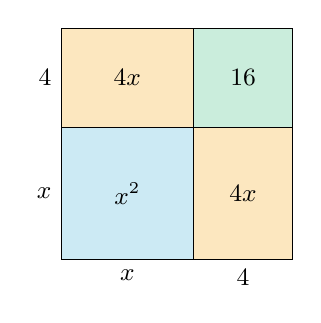
\begin{tikzpicture}[scale=0.42,font=\small]
\fill[fmkey!20] (0,0) rectangle (4,4); \fill[fmturn!25] (4,0) rectangle (7,4); \fill[fmturn!25] (0,4) rectangle (4,7); \fill[fmwatch!25] (4,4) rectangle (7,7);
\draw (0,0) rectangle (7,7); \draw (4,0)--(4,7); \draw (0,4)--(7,4);
\node at (2,2) {$x^2$}; \node at (5.5,2) {$4x$}; \node at (2,5.5) {$4x$}; \node at (5.5,5.5) {$16$};
\node[below] at (2,0) {$x$}; \node[below] at (5.5,0) {$4$}; \node[left] at (0,2) {$x$}; \node[left] at (0,5.5) {$4$};
\end{tikzpicture}\end{minipage}\end{watchme}
\begin{mistakebox}
$(x + 4)^2 \neq x^2 + 16$. \ Don't forget the middle term $2ab$: \ $(x + 4)^2 = (x+4)(x+4) = x^2 + 8x + 16$.\par
The last term is always \textbf{positive}: \ $(x - 3)^2$ ends in $+9$, not $-9$.
\end{mistakebox}
\needspace{2.4cm}\par\vspace{3mm}\noindent\begin{minipage}[t]{0.48\linewidth}{\color{fmturn}\bfseries 6.}\ Expand: \ $(x + 3)^2$\par\vspace{1.4cm}\hfill\rule{4.2cm}{0.4pt}\end{minipage}\hfill\begin{minipage}[t]{0.48\linewidth}{\color{fmturn}\bfseries 7.}\ Expand: \ $(x - 4)^2$\par\vspace{1.4cm}\hfill\rule{4.2cm}{0.4pt}\end{minipage}\par
\needspace{2.4cm}\par\vspace{3mm}\noindent\begin{minipage}[t]{0.48\linewidth}{\color{fmturn}\bfseries 8.}\ Expand: \ $(x + 5)^2$\par\vspace{1.4cm}\hfill\rule{4.2cm}{0.4pt}\end{minipage}\hfill\begin{minipage}[t]{0.48\linewidth}{\color{fmturn}\bfseries 9.}\ Expand: \ $(2x + 1)^2$\par\vspace{1.4cm}\hfill\rule{4.2cm}{0.4pt}\end{minipage}\par
\needspace{2.4cm}\par\vspace{3mm}\noindent\begin{minipage}[t]{0.48\linewidth}{\color{fmturn}\bfseries 10.}\ Expand: \ $(x - 6)^2$\par\vspace{1.4cm}\hfill\rule{4.2cm}{0.4pt}\end{minipage}\hfill\begin{minipage}[t]{0.48\linewidth}\ \end{minipage}\par
\needspace{9cm}\topicbar{Type 3 \quad Sum Times Difference: $(a+b)(a-b)$}
\begin{watchme}\textbf{Pattern:} \quad $(a + b)(a - b) = a^2 - b^2$ \quad (``difference of squares'')\par\vspace{2mm}
\textbf{Expand} \ $(x + 6)(x - 6)$.\par
\quad FOIL: \ $x^2 - 6x + 6x - 36$. \ The middle terms \textbf{cancel}! \ $\Rightarrow \ \boldsymbol{x^2 - 36}$\par
\quad Pattern: \ $a = x$, $b = 6$: \ $x^2 - 6^2 = \boldsymbol{x^2 - 36}$\par\vspace{1mm}
\textit{Order does not matter:} $(x - 6)(x + 6)$ gives the same answer. \ \textit{With a coefficient:} $(2x + 1)(2x - 1) = (2x)^2 - 1^2 = 4x^2 - 1$.\end{watchme}
\needspace{2.2cm}\par\vspace{3mm}\noindent\begin{minipage}[t]{0.48\linewidth}{\color{fmturn}\bfseries 11.}\ Expand: \ $(x + 5)(x - 5)$\par\vspace{1.2cm}\hfill\rule{4.2cm}{0.4pt}\end{minipage}\hfill\begin{minipage}[t]{0.48\linewidth}{\color{fmturn}\bfseries 12.}\ Expand: \ $(x - 7)(x + 7)$\par\vspace{1.2cm}\hfill\rule{4.2cm}{0.4pt}\end{minipage}\par
\needspace{2.2cm}\par\vspace{3mm}\noindent\begin{minipage}[t]{0.48\linewidth}{\color{fmturn}\bfseries 13.}\ Expand: \ $(2x + 3)(2x - 3)$\par\vspace{1.2cm}\hfill\rule{4.2cm}{0.4pt}\end{minipage}\hfill\begin{minipage}[t]{0.48\linewidth}{\color{fmturn}\bfseries 14.}\ Expand: \ $(x + 10)(x - 10)$\par\vspace{1.2cm}\hfill\rule{4.2cm}{0.4pt}\end{minipage}\par
\needspace{2.2cm}\par\vspace{3mm}\noindent\begin{minipage}[t]{0.48\linewidth}{\color{fmturn}\bfseries 15.}\ Expand: \ $(3x - 1)(3x + 1)$\par\vspace{1.2cm}\hfill\rule{4.2cm}{0.4pt}\end{minipage}\hfill\begin{minipage}[t]{0.48\linewidth}\ \end{minipage}\par\end{document}